\chapter{Introduction}
\label{chap:intro}
% \subsection*{Geodata \& Geodata computation}

The field of \ac{GIS} concerns itself with the collection, processing, storage, and visualization of geodata. 
By doing so, we offer the world priceless information about the land we build on, the seas we traverse, the air we breath, and the climates we inhabit. 
This information is foundational for many applications, including environmental modelling, infrastructure, urban planning, governance, navigation, the military, and agriculture.   

Central to these goals is \ac{geocomputation}. 
The term geocomputation, or geodata processing, is used to represent all types of computations performed on geographical datasets. Anything from the calculation of the area of a region, to a \ac{CRS} transformations, or converting a raster dataset into a vectorized dataset, can be regarded as geocomputation.

geocomputation is a cornerstone of \ac{GIS}, and vital to almost all its applications.
In the field of GIS, the raw \emph{data} gathered from direct land surveyance (e.g. terrain height samples) seldom equals to the precise \emph{information} we wish to discover about the earth (e.g. is my city in risk of flooding?).
To convert data into more rich information, a refinement and analysis process by means of geocomputation is required. 
Geocomputation is also necessary for specializing geodata. 
For example, various computations are needed for converting raw cadastral records into a base map useful to urban planners.

Despite major advancements during the last decades in geocomputation and geocomputation platforms, geocomputation remains no trivial exercise. 
The geometric nature of geocomputation, together with the sheer scope of geodata and the variety in formats and quality, make geocomputation both computationally intensive and difficult to operate. 

While researchers and developers have made considerable improvement over the last \\ decades, the improvement of both geocomputation, and the activity of geocomputation, remains as relevant as ever before. 

In recent years, a new development regarding geocomputation is emerging:
browser-based geocomputation by means of a \ac{VPL}.
The goal of this study is to contribute to this development. 
However, to specify its contribution, an explanation of this method must first be given.

\subsection*{The (web) VPL}

\begin{figure}
  \centering
  \graphicspath{{../../assets/images/background/geo-vpl/}}
  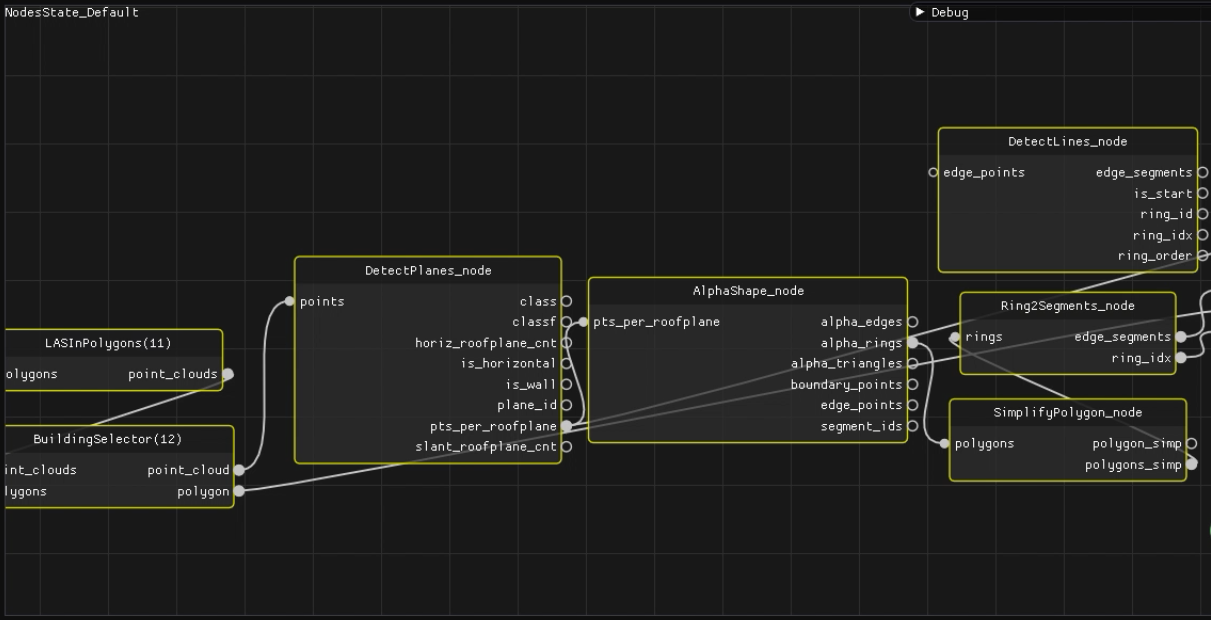
\includegraphics[width=\linewidth]{geoflow.png}
  \caption{Geoflow: A geocomputation VPL. \citep{peters_geoflow_2019}}
  \label{fig:1:geoflow}
\end{figure}

% from :  Conal Elliott
% tangible values

% libraries 
% means to an end

% applications 
% the end (dead end)



% The split has drawbacks: 
% - Applications limit access to functionalities 
% - Applications are ususally not composable

% - Libraries have limited access and usage.
% - The medium affects

% The dream: 
% - unlimited access to functionality & composability, usability, and composability

A visual programming language is a type of programming language which uses an alternative model to the textual source code of regular programming languages. 
These alternative models are represented by a \ac{GUI}, in which the program might take the shape of a graph or a block-based instruction set for example. 
The value a VPL lies in the fact that constructing or editing a program in a visual way can be a faster process than using a textual method, even for the most experienced software developers \citep{green_usability_1996, kuhail_characterizing_2021}.
Additionally, a \ac{VPL} allows for End User Development \citep{kuhail_characterizing_2021}: 
In general, \ac{VPL} makes processes more accessible to end users, as it allows practitioners to automate some processes and workflows like a software developer, but without needing a full background in software development \citep{benac_recent_2022}. 
Finally, VPLs may even possess performance and reliability advantages over textual languages, but only if it is implemented as a so-called dataflow-type VPL \citep{sousa_dataflow_2012}. 

These qualities are beneficial to geocomputation, and perhaps as a consequence, geocomputation by means of visual programming is not an uncommon phenomena in the field of \ac{GIS}.
For example, Safe software's FME \citep{safe-software_fme_2022} is a popular \ac{VPL} among \ac{GIS} practitioners, arguably due to the way it simplifies the process of writing a \ac{ETL} pipeline. 
Another example is McNeel's Grasshopper \citep{rutten_grasshopper_2012}, often used for small-scale spatial analyses, like solar irradiation or heating demands of a neighborhood \citep{sadeghipour_roudsari_ladybug_2013}. 

A new development regarding Geocomputation VPLs is attempting to make these VPLs run in a web browser.
The value of this is that web applications require no explicit installment to use the application, giving them distribution and accessibility advantages over native applications \citep{kuhail_characterizing_2021, panidi_hybrid_2015}. 
The Mobius Modeller is a good example of a browser-based geocomputation VPL \citep{janssen_mobius_2021}.
The application allows users to configure a calculation by visual means in a web browser, which can then be shared as a stand-alone web application. 

%%%%%%%%%%%%%%%%%%%%%%%%%%%%%%%%%%%%%%%%%%%%%%%%%%%%%%%%%%%%%%%%%%%%%%%%%%%%%%%

% \subsection*{Shortcoming: No true dataflow programming}

% The assumption that a geo-web-vpl should be implemented as a dataflow vpl is made because of the many advantageous qualities layed out in \refsec{sec:background:dataflow}. 
% Additionally, and perhaps consequently, all comparable VPLs analyzed in \refsec{sec:related-geovpl} were implemented as dataflow VPLs (Blender, houdini, Grasshopper, GeoFlow), the only exception being the Möbius Modeller.
% However, this meant that a new, web-based implementation had to be made, since no existing web-vpl concerned with geometry uses this model (that this study is aware of).

\subsection*{Problem Statement}
  
The web based geocomputation VPL is a novel development, and contains a multitude of unaddressed challenges.
This study focusses on the particular problem of library portability. % and integration

Successful geocomputation pipelines often relies on operations found in a select number of libraries. 
Most major, industry-standard geocomputation libraries are native, C++-based libraries. 
Examples of these are GDAL, PROJ, and GEOS. 
However, A web based geocomputation VPL like the Mobius Modeller does not make use of these libraries, and uses javascript equivalents like Turf \citep{turf_contributors_turfjs_2022}.
While it is possible to port a library like GDAL to javascript, guarantying that these two versions show the same behavior will be complex and time consuming. Additionally, managing duplicate libraries like this will slow down development, or create large version discrepancies \citep{ammann_maplibre-rs_2022}.

Fortunately, on a theoretical level, it is possible to compile a native C++ library to a web-consumable format using the 'WebAssembly' binary format \citep{haas_bringing_2017}.
This way, only one library needs to be maintained to serve all platforms, both native and web. 
However, to the best of the author's knowledge, no example exists of a web-based geocomputation VPLs which make use of native geocomputation libraries.
The theoretical possibility combined with the practical absence of any implementation, leads this study to assume that a practical inhibition is in place, preventing native geocomputation libraries to be used by a web VPL.

The source of this inhibition is unclear. 
There are many aspects and components to compiling a native geocomputation library, and using it on the web, in a VPL format. 
Given the absence of an implementation, the possibility remains that it could be any one of these aspects and components, or even an interplay between all of these factors. 
This study identifies three main challenges to using a native geocomputation library in a web-based VPL:

\subsubsection*{\mySubRQTwoTitle}

% Secondly, native geocomputation functionalities might not be able to be properly \textbf{compiled} into a format functional on the web.
% (wasm limitations)

% Making sure a \ac{geo-web-vpl} is able to make use of native, system-level libraries is a key component, since it will mean access to powerful, industry standard geocomputation libraries like CGAL and GDAL. 
Firstly, the challenge of compilation. 
As explained before, the most viable option for using a non-js library in a web browser, is by compiling it to WebAssembly \citep{haas_bringing_2017}.
Other options exist, like simply rewriting non-js languages to JavaScript, but these methods have significant drawbacks \citep{haas_bringing_2017,jangda_not_2019}.
However, as described in \refsec{sec:related-geoweb} compiling libraries to \ac{wasm} also may pose challenges:

% The study starts out with the assumption that WebAssembly must be utilized to properly compile and run existing geoprocessing libraries in a browser. This might not be as easy as using normal compilers, based on the experience gained by preliminary work (See \autoref{sec:preliminary-wasm}). WebAssembly is containerized and makes no assumptions about its source language \cite{haas_bringing_2017}, making aspects such as an SDK, sub-dependencies called using environment variables, and IO (file reading and writing) possible obstacles. 

\begin{enumerate}[-]
  \item \ac{wasm} promises a 'near native performance' \citep{haas_bringing_2017}. However, this can be quite situational, as multiple studies have shown \citep{jangda_not_2019, melch_performance_2019}. 
  \item \ac{wasm} cannot compile all code. Its containerized nature means that code accessing a file system for example, does not function without workarounds. 
  \item Compiled \ac{wasm} code could be difficult to access and interface in a web browser. Without third-party tools, functions exposed by \ac{wasm} can only accept primitive data types as input. There is no \m{string} data type, let alone a \m{struct} or \m{object} type. 
  \item Compiling an \emph{library} to \ac{wasm} is seriously different from compiling a full \emph{application} to wasm. A library requires more complicated wasm-javascript interoperability, which third-party tools may or may not be able to provide.
\end{enumerate}
% Discovering the extent and relevance of these compilation challenges for geo-computation libraries is why the sub-question of \mySubRQTwoTitle \space was included in this study.

\subsubsection*{\mySubRQThreeTitle}

Secondly, even if the libraries are compiled to a web-ready format, geocomputation functionalities might not be able to \textbf{load} properly within a web-based VPL.

This is a challenge of designing an appropriate binding system or plugin loader. 
When writing Python bindings to a C++ library for example, one has to consider the way both languages operate, and make sure the discrepancies between the language models are accounted for, such as manual memory management. 
This is not different from a visual language interfacing with a web-compiled native library. 
However, this situation adds additional challenges, as the host \ac{VPL} does not necessarily know the source language of the binary. 


% This is a matter of bindings, 
\subsubsection*{\mySubRQFourTitle}

Finally, It might be the case that a web-based VPL \emph{is} able to load and run functions from native, non-js geo-computation libraries. 
And still, one might not be able to successfully \textbf{use} these libraries.

Central to this challenge of utilization is the aforementioned dataflow VPL format. 
The performance and reliability needed for geocomputation makes a strong argument that any geocomputation VPL should be implemented as a dataflow VPL. 
This is also evident from the fact that almost all geocomputation and geometry manipulation VPLs are implemented as a dataflow VPL (see \refsec{sec:related-geovpl}).

However, it may be that native geocomputation functionalities are unfit for this model. 
The model requires all functions to be pure, and all variables to be immutable. 
This might invalidate some of the operations found in these libraries, or make other operations complicated to use in practice.


\section{Research Objective}
This study seeks to improve the state of browser-based geocomputation VPLs.
This is done by studying a possible solution to the library portability problem found in existing browser-based geocomputation VPLs.

The study poses that the library portability problem can only be overcome if native geocomputation libraries are able to be properly compiled, loaded and utilized in a browser-based dataflow-VPL format. 
There are multitude of technical challenges present within each one of these steps, and in between these steps. 
Seeking and analyzing solutions to these challenges is the focal point of this study. 


\section{Research Questions}
Based on this objective, the research question is formulated as follows: 
\begin{itemize}[ ]
  \item \myMainRQ
\end{itemize}


\subsection*{Supporting Questions}
The following supporting questions are defined to aid in answering the main question.
The first question serves as a prerequisite for attempting to answer the remaining three. 
The other three research questions are based upon the three main categories of challenges of the library portability problem.  
These questions are posed in such a way that answering them will require us to explore the extent of this challenge, and find possible solutions.


\begin{itemize}[-]
  \item \mySubRQOne
  \item \mySubRQTwo
  \item \mySubRQThree
  \item \mySubRQFour
\end{itemize}

\subsection*{Evaluation}
In order to obtain answers to these questions, a literature review is performed,
a prototype web-based geocomputation VPL is developed, 
and this application is accessed on various aspects.

This prototype vpl is both used as a test case to discover the extent of possible challenges, as well as a staging ground for possible solutions. 
The specific way in which each sub-research question is evaluated is explained in \refchap{chap:methodology}.

% \begin{note}
% TODO: diagram: 4 research questions -> four possible barriers of geocomputation
% \end{note}

% \begin{note}
% TODO: diagram: show the 'locations' of the four research questions ( client / server / native, etc.)
% \end{note}

% \subsection*{Nature}
% The methodology of this study can be characterized as practical as opposed to theoretical, 
% % wholistic instead of specific, 
% and iterative compared to linear. 
% The prior works on browser-based geocomputation and geo-vpls indicate that a strong theoretical framework for a \ac{geo-web-vpl} is in place (Source). 
% But, and this is especially evident in the prior studies regarding Browser-based geocomputation, the practical implementation of these theories were only partially successful, and limited in scope. 
% This necessitates a practical approach in response. 
% And, due to the investigative nature of this study, the methodology requires to iterate upon itself, instead of following a singular, linear path. 

% MIGHT NOW WANT TO KEEP THIS IN HERE
% ...
% % Theorie: is er maar je geloofde het niet
% % praktische implementatie om de Throerie weerleggen
% The prior works on browser-based geoprocessing indicate that a theoretical framework for browser-based geoprocessing vpl is in place. 
% But, and this is especially evident in the studies regarding client-side geoprocessing, the practical implementation of these theories

% Choices: 
% - practical > theoretical : Literature study indicates enough theoretical soundness, but lots of practical questions remaining. We wish to  immediate pick up where these studies have left, and therefore we choose the direct, practical study of designing and implementing a prototype application. 
% - wholistic > specific    : Research in one sub-domain could have been more exhaustive in one of the specific sub-studies, instead of covering the full scope it does now. However, This would have been incomplete. What we do now is cover the full pipeline of using a geocomputation library: from creation to web export, to web import, to web utilization. by doing this, we can identify issues caused in one of these
% - iterative > linear      : Given this vast scope, many questions can come up from different angles. The study has to be dynamic to adapt to these demands. 

\newpage
\section{Scope}
The scope of this thesis is bounded in the following seven ways: 

\subsection*{Only frontend geocomputation}

% \begin{note}
%   [KEN]: p.5 is backend geocomputation really browser-based geocomputation? I'd say no, could be used to shorten this section

%   [JOS]: I would still include this part, when I explain my thesis to colleagues and other people, the difference between 'web-based geocomputation' and 'browser-based' comes up. Better safe than sorry.
%   I have, however, trimmed this section down a bit
% \end{note}

There is a nuance between 'web-based geocomputation' and 'browser-based geocomputation'. 
'Web' can refer to both frontend and backend computation methods, 'browser' refers purely to frontend computations. 
This study focusses on browser-based geocomputation, and as such, excludes any \emph {backend} based geocomputation.
% A web application \textit{could} be used to orchestrate geocomputation web-services, which could also deliver a form of browser-based geocomputation to end-users. 
% However, for the scope of this thesis, we limit ourselves to purely client-side solutions, with calculations literally happening within the clients browser. 
% This is also why this study excludes the OGC standard of the \ac{WPS} \cite{ogc_web_2015}.

Adding backend-based geocomputation to a web VPL would be an excellent follow-up investigation to this study, following in the footsteps of studies like \cite{panidi_hybrid_2015}. 

\subsection*{No Usability Comparison} % 

While accessibility / usability is a motivation of the development of a \ac{VPL}, and while usability will be analyzed to a limited extent, no claims will be made that this method of geocomputation is \emph{more} usable as opposed to existing geocomputation methods. 
This research attempts to solve practical inhibitions in order to discover whether or not browser-based, vpl-based geocomputation is \emph{a} viable, usable option. If it turns out that this method is viable enough technically, future research will be needed to definitively proof \emph{how} usable it is compared to all other existing methods. 
Similarly, a survey analyzing how users experience browser-based geocomputation in comparison to native geocomputation must also be left to subsequent research. 

This choice is made, because browser-based, VPL-based geocomputation is too new of a method to make a balanced comparison against any other method. Native environments like QGIS, FME or ArcGIS simply have a twenty year lead in research and development. 

% This paper seeks to first close this gap, limiting itself to overcoming the technical and design boundaries in the pursuit of practical client-side geocomputation.

% While the research restrains itself from empirically measuring an aspect as nebulous as 'accessibility', it does demonstrate ...


% It is my goal to introduce this as a new geocomputation option, and to name the advantages and disadvantages we can be sure of. An actual comparison of client-side vs native geocomputation is something different. 

\subsection*{Only WebAssembly-based containerization}

This thesis examines a WebAssembly-based approach to containerization and distribution of geocomputation functionalities. 
Containerization using Docker is also possible for server-side applications, but is not (easily) usable within a browser. 
For this reason, Docker-based containerization is left out of this studies' examination. 
And to clarify: Docker and WebAssembly are not mutually exclusive models, and could be used in conjunction on servers or native environments. 

\subsection*{Mostly Point Cloud/ DTM focussed geocomputation}

We are also required to concentrate the scope of 'geocomputation', which is a sizable phenomenon.
The term is generally used to cover all operations on geodata, from rasters, tabular datasets, highly structured datasets such as the CityJSON or IndoorGML, and point clouds. 
Due to time limitations, we are forced to focus on particular type of geocomputation.
3D-based geocomputation is chosen, with a particular focus on pointclouds and DTMs. 
The hypothesis is that these types of data may fit the small-scale geocomputation of a VPL well due to the local optimality quality of many DTM procedures (Such as the \ac{DT}), 

\subsection*{Assumption: a 'Geocomputation-VPL' is a Geometry VPL able to handle geodata}
For the scope of this thesis, we assume a VPL for geocomputation is practically the same as a VPL for generic geometry processing.
Examples of "Geometry VPLs" are Blender's Geometry Nodes, Houdini, and Grasshopper.
More on this in chapter \refsec{sec:related-geovpl}.

A Geocomputation VPL differs only in the fact that it supports additional geodata types, and offers functionalities specific to processing those types.  
This assumption is safe to make since a geocomputation VPL will \emph{at the very least} require the same features as a 'normal' geometry VPL, due to their common dependency on the field of computer graphics and computational geometry.

Still, in reality, a lot of differences and nuances exist between the field of geocomputation and the field of procedural modelling. 
However, due to time limitations, these concerns are left to future research.
% these concerns will only be picked up at the final discussion, found at \refsec{sec:discussion}.
 
\subsection*{Only geocomputation libraries written in C++ \& Rust}
The study limits itself to native libraries written in C++ and Rust. 
C++ was chosen, since almost all relevant geocomputation libraries are written in C++, like CGAL and PROJ. 
Rust was chosen, for its extensive WebAssembly support. 
It also appears to be the most popular language for writing WebAssembly \citep{eberhardt_state_2022}.
It contains a number of relevant geocomputation libraries, but not to the same extend as C++.

\subsection*{Only core browser features}
Lastly, the implementation of the prototype geocomputation VPL will limit itself to core browser features, keeping dependencies at a minimum, in an attempt to generalize the results of the study.
If the study would use specific web frameworks and technologies to solve key issues, questions might arise if the results of the study counts in general for browser-based geocomputation or geocomputation VPLs, or if they only count in this specific scenario. 
"Core browser features" is defined in \refsec{sec:method:base-vpl}.

\newpage
\section{Reading Guide}
The remainder of this study is structured as follows:


\begin{itemize}[ ]
  \item \refchap{chap:background}, Background, provides an overview of the theoretical background that is used in the rest of this study.
  
  \item \refchap{chap:related}, Related Work, provides a review of studies comparable to this one.

  \item \refchap{chap:methodology}, Methodology, explains precisely in what way the research-questions will be answered.
  In addition, the main design decisions are described and justified in this part of the study.

  \item \refchap{chap:implementation}, Implementation, presents the implementation of the methodology.
  
  \item \refchap{chap:testing}, Testing, tests the results from this implementation in various ways described by the methodology.
  
  \item And finally, \refchap{chap:conclusion}: Conclusion \& Discussion, concludes to which extent the study was able to satisfy the main research question, and discusses unaddressed aspects of the thesis.
  It also includes the envisioned future works and a reflection on the quality of the study.

\end{itemize}